\documentclass[10pt]{beamer}

\usetheme{default}

\usepackage[utf8]{inputenc}
\usepackage[russian]{babel}
\usepackage[OT1]{fontenc}
\usepackage{amsmath}
\usepackage{amsfonts}
\usepackage{amssymb}
\usepackage{graphicx}
\usepackage{etoolbox}
\usepackage{caption}
\usepackage{subcaption}
\usepackage{pifont}
\usepackage{xcolor}
\usepackage{framed}
\definecolor{shadecolor}{cmyk}{0,0,0,1}
\usepackage{multirow}

\usepackage{listings}

\lstset{
	backgroundcolor=\color{lightgray},
	commentstyle=\color{blue},
	frame=single
	breakatwhitespace, 
	language=python, 
	columns=fullflexible, 
	keepspaces, 
	breaklines, 
	tabsize=3, 
	showstringspaces=false, 
	extendedchars=true,
	numbers=left
}

\makeatletter

\setbeamercolor{title}{fg=white}
\setbeamercolor{frametitle}{fg=black}
\setbeamerfont*{title}{family=\sffamily,size=\LARGE}

\setbeamerfont{page number in head/foot}{size=\scriptsize}
\setbeamertemplate{footline}[frame number]
\let\otp\titlepage
\renewcommand{\titlepage}{\otp\addtocounter{framenumber}{-1}}

\setbeamertemplate{background canvas}{%
	\ifnumequal{\c@framenumber}{0}{%
      
\includegraphics[width=\paperwidth,height=\paperheight]{images/cover.png}
   }{%
      \ifnumequal{\c@framenumber}{\inserttotalframenumber}{
         
\includegraphics[width=\paperwidth,height=\paperheight]{images/back.png}
      }{%
         % Other frames
      }%
   }%
}

\makeatother

\beamertemplatenavigationsymbolsempty

\author{Николай Анохин}
\title{\newline \newline \newline Лекция 4 \\ Задача классификации}

\begin{document}

\begin{frame}[plain]
\titlepage
\end{frame}

\begin{frame}{План занятия}
\tableofcontents
\end{frame}

% ========================================
\section{Задачи классификации и регрессии}
% ========================================

\begin{frame}{}

\begin{center}
\Large Задачи классификации и регрессии
\end{center}

\end{frame}

\begin{frame}{Классификация: интуиция}

\begin{block}{Задача}
Разработать алгоритм, позволяющий определить класс произвольного объекта из некоторго множества
\begin{itemize}
\item Дана {\it обучающая выборка}, в которой для каждого объекта известен класс
\end{itemize}
\end{block} 

\begin{center}
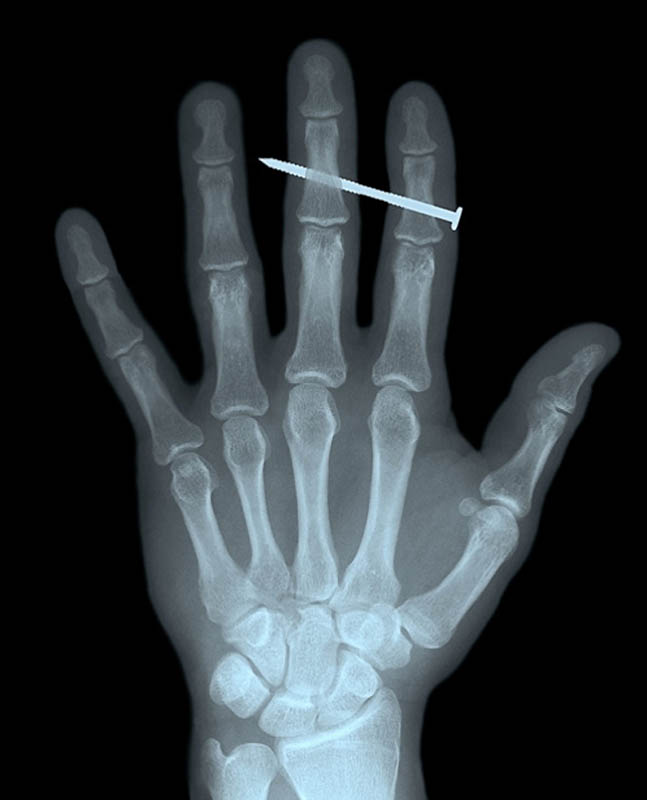
\includegraphics[scale=0.15]{images/xray.jpg}
\end{center}

\end{frame}

\begin{frame}{Регрессия: интуиция}

\begin{block}{Задача}
Разработать алгоритм, позволяющий предсказать числовую характеристику произвольного объекта из некоторого множества
\begin{itemize}
\item Дана {\it обучающая выборка}, в которой для каждого объекта известно значение числовой характеристики
\end{itemize}
\end{block}

\begin{center}
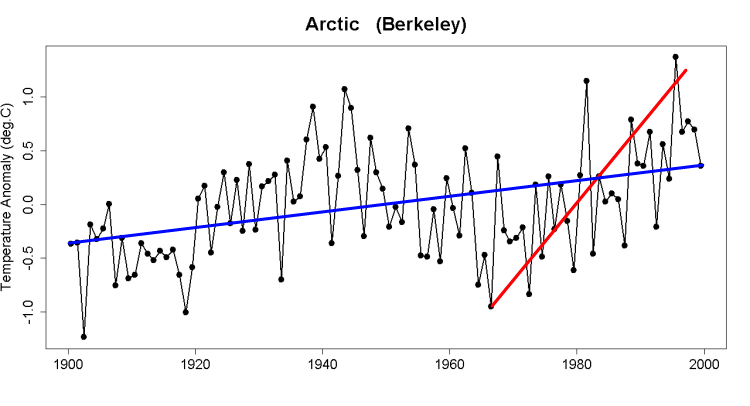
\includegraphics[scale=0.3]{images/kioto.png}
\end{center}

\end{frame}

\begin{frame}{Постановка задачи}

Пусть дан набор объектов $\mathcal{D} = \{(\mathbf{x}_i, y_i)\},
\; \mathbf{x}_i \in \mathcal{X},
\; y_i \in \mathcal{Y},
\; i \in 1, \ldots, N$, полученный из неизвестной закономерности $y = f(\mathbf{x})$. Необходимо выбрать из семейства параметрических функций
\[
H = \{h(\mathbf{x}, \theta): \mathcal{X} \times \Theta \rightarrow \mathcal{Y} \}
\]
такую $h^*(\mathbf{x}) = h(\mathbf{x}, \theta^*)$, которая наиболее точно апроксимирует $f(\mathbf{x})$.

\vspace{1em}
Задачи
\begin{itemize}
\item Классификация: $|\mathcal{Y}| < C$
\item Регрессия: $\mathcal{Y} = [a, b] \subset \mathbb{R}$
\end{itemize}

\end{frame}

\begin{frame}{Как решать}

\begin{enumerate}

\item[M] Выдвигаем гипотезу насчет {\bf модели} - семейства параметрических функций вида
\[
H = \{h(\mathbf{x}, \theta): \mathcal{X} \times \Theta \rightarrow \mathcal{Y} \},
\]
которая могла бы решить нашу задачу (model selection)

\item[L] Выбираем наилучшие параметры модели $\theta^*$, используя {\bf алгоритм обучения}
\[
A(X, Y) : (\mathcal{X}, \mathcal{Y})^N \rightarrow \Theta
\]
(learning/inference)

\item[D] Используя полученную модель $h^*(\mathbf{x}) = h(\mathbf{x}, \theta^*)$, классифицируем неизвестные объекты (decision making)

\end{enumerate}

\end{frame}

% ========================================
\section{Подходы к моделированию}
% ========================================

\begin{frame}{}

\begin{center}
\Large Подходы к моделированию
\end{center}

\end{frame}

\begin{frame}{Виды моделей}

{\bf Генеративные модели.} Смоделировать $p(\mathbf{x} | y_k)$ и $p(y_k)$, применить теорему Байеса
\[
p(y_k | \mathbf{x}) = \frac{p(\mathbf{x} | y_k) p(y_k)}{p(\mathbf{x})}
\]
и использовать $p(y_k | \mathbf{x})$ для принятия решения \\ (NB, Bayes Networks, MRF)
\vspace{1em}

{\bf Дискриминативные модели.} Смоделировать $p(y_k | \mathbf{x})$ и использовать ее для принятия решения \\ (Logistic Regression, Decision Trees)
\vspace{1em}

{\bf Функции решения.} Смоделировать напрямую $h^*(\mathbf{x}): \mathcal{X} \rightarrow \mathcal{Y}$ \\ (Linear Models, Neural Networks)

\end{frame}

\begin{frame}{Вероятностные модели VS Функции решения}

\begin{itemize}
\item[\color{green}\ding{108}] Отказ от классификации (reject option)
\item[\color{green}\ding{108}] Дисбаланс в выборке
\item[\color{green}\ding{108}] Ансамбли моделей
\item[\color{red}\ding{108}] Сильные предположения о природе данных
\item[\color{red}\ding{108}] Излишняя (вычислительная) сложность
\end{itemize}

\end{frame}

\begin{frame}{Байесовский подход к моделированию}

{\bf Идея.} Вместо фиксированного, но неизвестного $\theta^*$ ищем апостериорное распределение $p(\theta | \mathcal{D})$\\ 
{\bf Дано.} $p(y_i)$, $p(\theta)$, $p(\mathbf{x} | \theta)$ 
\[
p(y_i | \mathbf{x}, \mathcal{D})= \frac{p(\mathbf{x} | y_i, \mathcal{D}) p(y_i | \mathcal{D})}{\sum_jp(\mathbf{x} | y_j, \mathcal{D}) p(y_j | \mathcal{D})} = \frac{p(\mathbf{x} | y_i, \mathcal{D}) p(y_i)}{\sum_jp(\mathbf{x} | y_j, \mathcal{D}) p(y_j)}
\]
\[
p(\mathbf{x} | y_i, \mathcal{D}) = \int p(\mathbf{x} | \theta) p(\theta | \mathcal{D}) d\theta
\]
Апостериорное распределение
\[
p(\theta | \mathcal{D}) = \frac{p(\mathcal{D} | \theta) p(\theta)}{\int p(\mathcal{D} | \theta) p(\theta) d\theta} = \frac{\prod_n p(\mathbf{x}_n | \theta) p(\theta)}{\int \prod_n p(\mathbf{x}_n | \theta) p(\theta) d\theta}
\]

\end{frame}

\begin{frame}{Обучение модели}

\begin{quote}
\[
LEARNING = representation + evaluation + optimization
\]
\hfill Pedro Domingos
\end{quote}

Evaluation -- критерий, который оптимизируем
\begin{itemize}
\item эмпирический риск $\rightarrow \min$
\item KL-дивергенция $\rightarrow \min$
\item функция правдоподобия $\rightarrow \max$
\item information gain $\rightarrow \max$
\end{itemize}
Optimization -- как оптимизируем
\begin{itemize}
\item unconstrained (GD, Newton+)
\item constrained (linear programming, quadratic programming)
\end{itemize}

\end{frame}

\begin{frame}{Эмпирический риск}

{\bf Функция потерь} $\mathcal{L}(\mathbf{x}, y, \theta)$ - ошибка, которую для данного $\mathbf{x}$ дает модель $h(\mathbf{x}, \theta)$ по сравнению с реальным значением $y$
\vspace{1em}

{\bf Эмпирический риск} -- средняя ошибка на обучающей выборке
\[
Q(X, Y, \theta) = \frac{1}{N} \sum_{n=1}^N \mathcal{L}(\mathbf{x}_n, y_n, \theta)
\]
\vspace{1em}

{\bf Задача} -- найти значение $\theta^*$, минимизирующее эмпирический риск
\[
\theta^* = \theta^*(X, Y) = \text{argmin}_\theta Q(X, Y, \theta)
\]

\end{frame}

\begin{frame}{Некоторые функции потерь}

\begin{itemize}
\item Индикатор ошибки
\[
\mathcal{L}(\mathbf{x}, y, \theta) = 0 \text{\;if\;} h(\mathbf{x}, \theta) = y \text{\;else\;} 1
\]
\item Функция Минковского 
\[
\mathcal{L}(\mathbf{x}, y, \theta) = |y - h(\mathbf{x}, \theta)|^q
\]
Частные случаи: квадратичная $q = 2$, абсолютная ошибка $q = 1$
\item Hinge
\[
\mathcal{L}(\mathbf{x}, y, \theta) = \max(0, 1 - y \times h(\mathbf{x}, \theta))
\]
\item Информационная
\[
\mathcal{L}(\mathbf{x}, y, \theta) = - \log_2 p(y | \mathbf{x}, \theta)
\]
\begin{center}

\end{center}
\end{itemize}

\end{frame}

\begin{frame}{Проблема 1. Переобучение}

\begin{block}{Задача}
Аппроксимировать обучающую выборку полиномом $M$ степени
\end{block}

\begin{center}
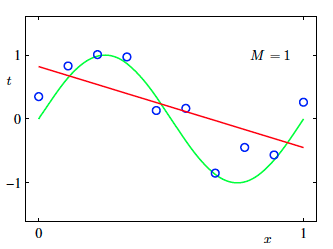
\includegraphics[scale=0.3]{images/m1.png}
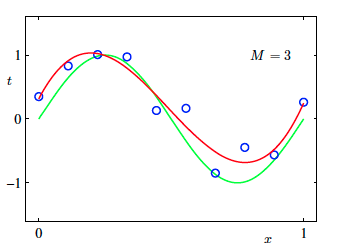
\includegraphics[scale=0.3]{images/m2.png}
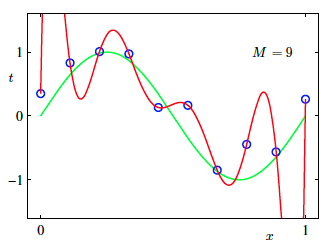
\includegraphics[scale=0.3]{images/m3.png}

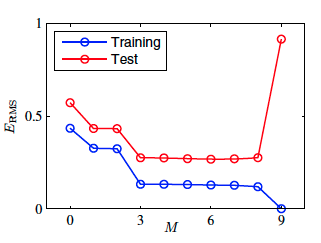
\includegraphics[scale=0.3]{images/of.png}
\end{center}

\end{frame}

\begin{frame}{Проблема 2. Проклятие размерности}

\begin{block}{Задача}
Классифицировать объекты.
\end{block}

\begin{center}
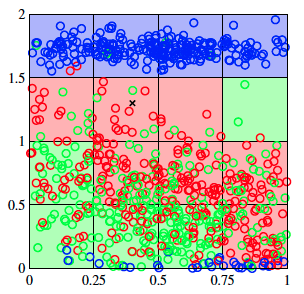
\includegraphics[scale=0.3]{images/pts.png}

\includegraphics[scale=0.4]{images/curse.png}
\end{center}

\end{frame}

% ========================================
\section{Теория принятия решений}
% ========================================

\begin{frame}{}

\begin{center}
\Large Теория принятия решений
\end{center}

\end{frame}

\begin{frame}{Классификация}

{\bf Пусть}

$\mathcal{R}_k$ -- область, такая что все $\mathbf{x} \in \mathcal{R}_k$ относим к $y_k$

{\bf Дано}

$R_{kj}$ -- риск, связанный с отнесением объекта класса $y_k$ к классу $y_j$

{\bf Найти}

$\forall k: \mathcal{R}_k$, такие, что математическое ожидание риска $E[R]$ минимально.

\[
E[R] = \sum_k \sum_j \int_{\mathcal{R}_j} R_{kj} p(y_k | \mathbf{x}) p(\mathbf{x}) dx
\]

\end{frame}

\begin{frame}{Медицинская диагностика}

Матрица риска $[R_{kj}]$

\begin{center}
\begin{tabular}{r | c c}
 & sick & normal \\
\hline
sick & 0 & 10 \\
normal & 1 & 0 
\end{tabular}
\end{center}

Условные вероятности $p(y_k | x)$
\[ 
p(\mathtt{normal} | \mathtt{moving}) = 0.9, \; p(\mathtt{normal} | {\mathtt{not\;moving}}) = 0.3
\]
Вероятности $p(x)$
\[
p(\mathtt{moving}) = 0.7
\]
Требуется определить $\mathcal{R}_{\mathtt{sick}}$, $\mathcal{R}_{\mathtt{normal}}$

\end{frame}

\begin{frame}{Регрессия}

Те же виды моделей: {\bf генеративные}, {\bf дискриминативные}, {\bf функция решения}
\vspace{1em}

Задана функция риска
\[
R(y, h(\mathbf{x}))
\]
Математическое ожидание $E[R]$
\[
E[R] = \int \!\! \int R(y, h(\mathbf{x})) p(\mathbf{x}, y) d\mathbf{x} dy
\]
Для квадратичной функции риска $R(y, h(\mathbf{x})) = [y - h(\mathbf{x})]^2$
\[
h(x) = E_y[h | \mathbf{x}] = \int y p(y | \mathbf{x}) dy
\]

\end{frame}

% ========================================
\section{Оценка результатов классификации}
% ========================================

\begin{frame}{}

\begin{center}
\Large Оценка результатов классификации
\end{center}

\end{frame}

\begin{frame}{Как оценить различные модели?}

\begin{block}{Идея}
использовать долю неверно классифицированных объектов \\ (error rate)
\end{block}

\begin{alertblock}{Важное замечание}
error rate на обучающей выборке {\bf НЕ} является хорошим показателем качества модели
\end{alertblock}

\end{frame}

\begin{frame}{Решение 1: разделение выборки}

Делим обучающую выборку на {\bf тренировочную}, {\bf валидационную} и {\bf тестовую}

\begin{center}
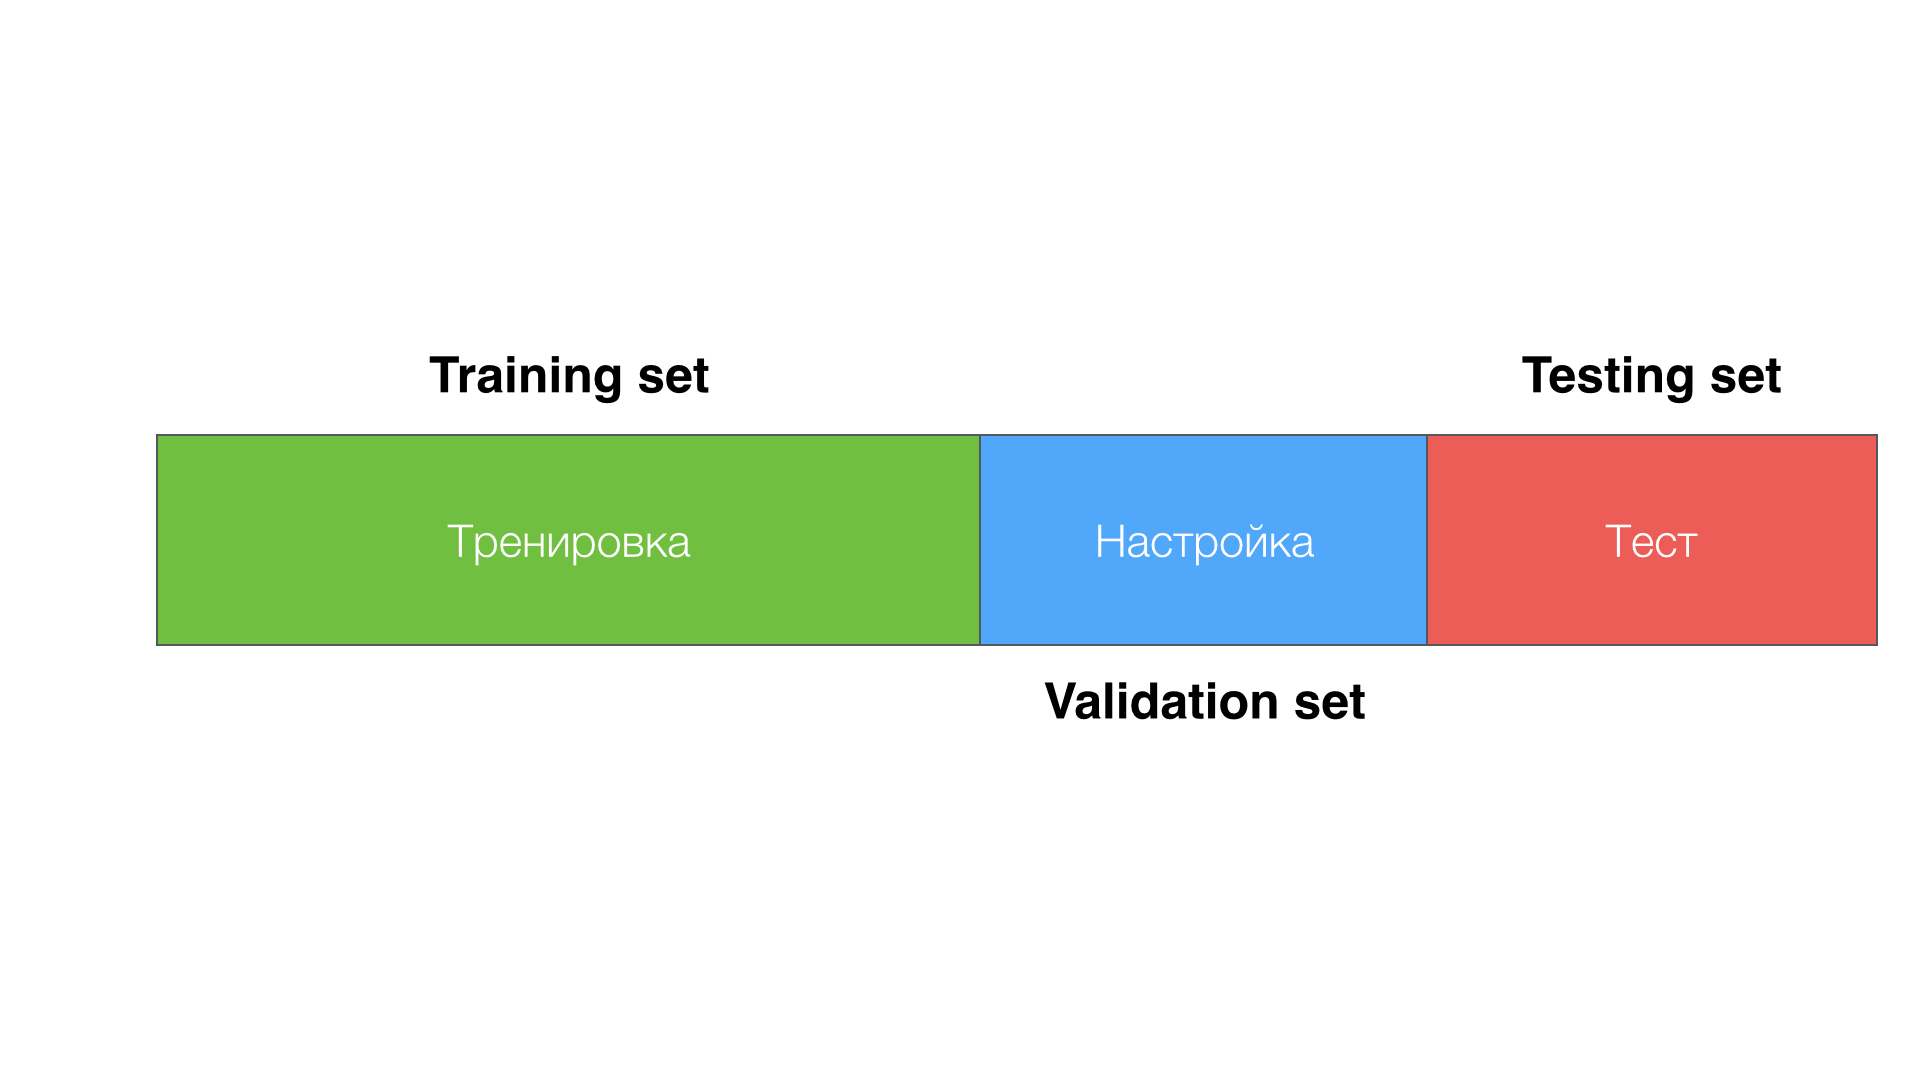
\includegraphics[scale=0.15]{images/vtt.png}
\end{center}
  
\end{frame}

\begin{frame}{Решение 2: скользящий контроль}

(n-times) (stratified) cross-validation

\begin{center}
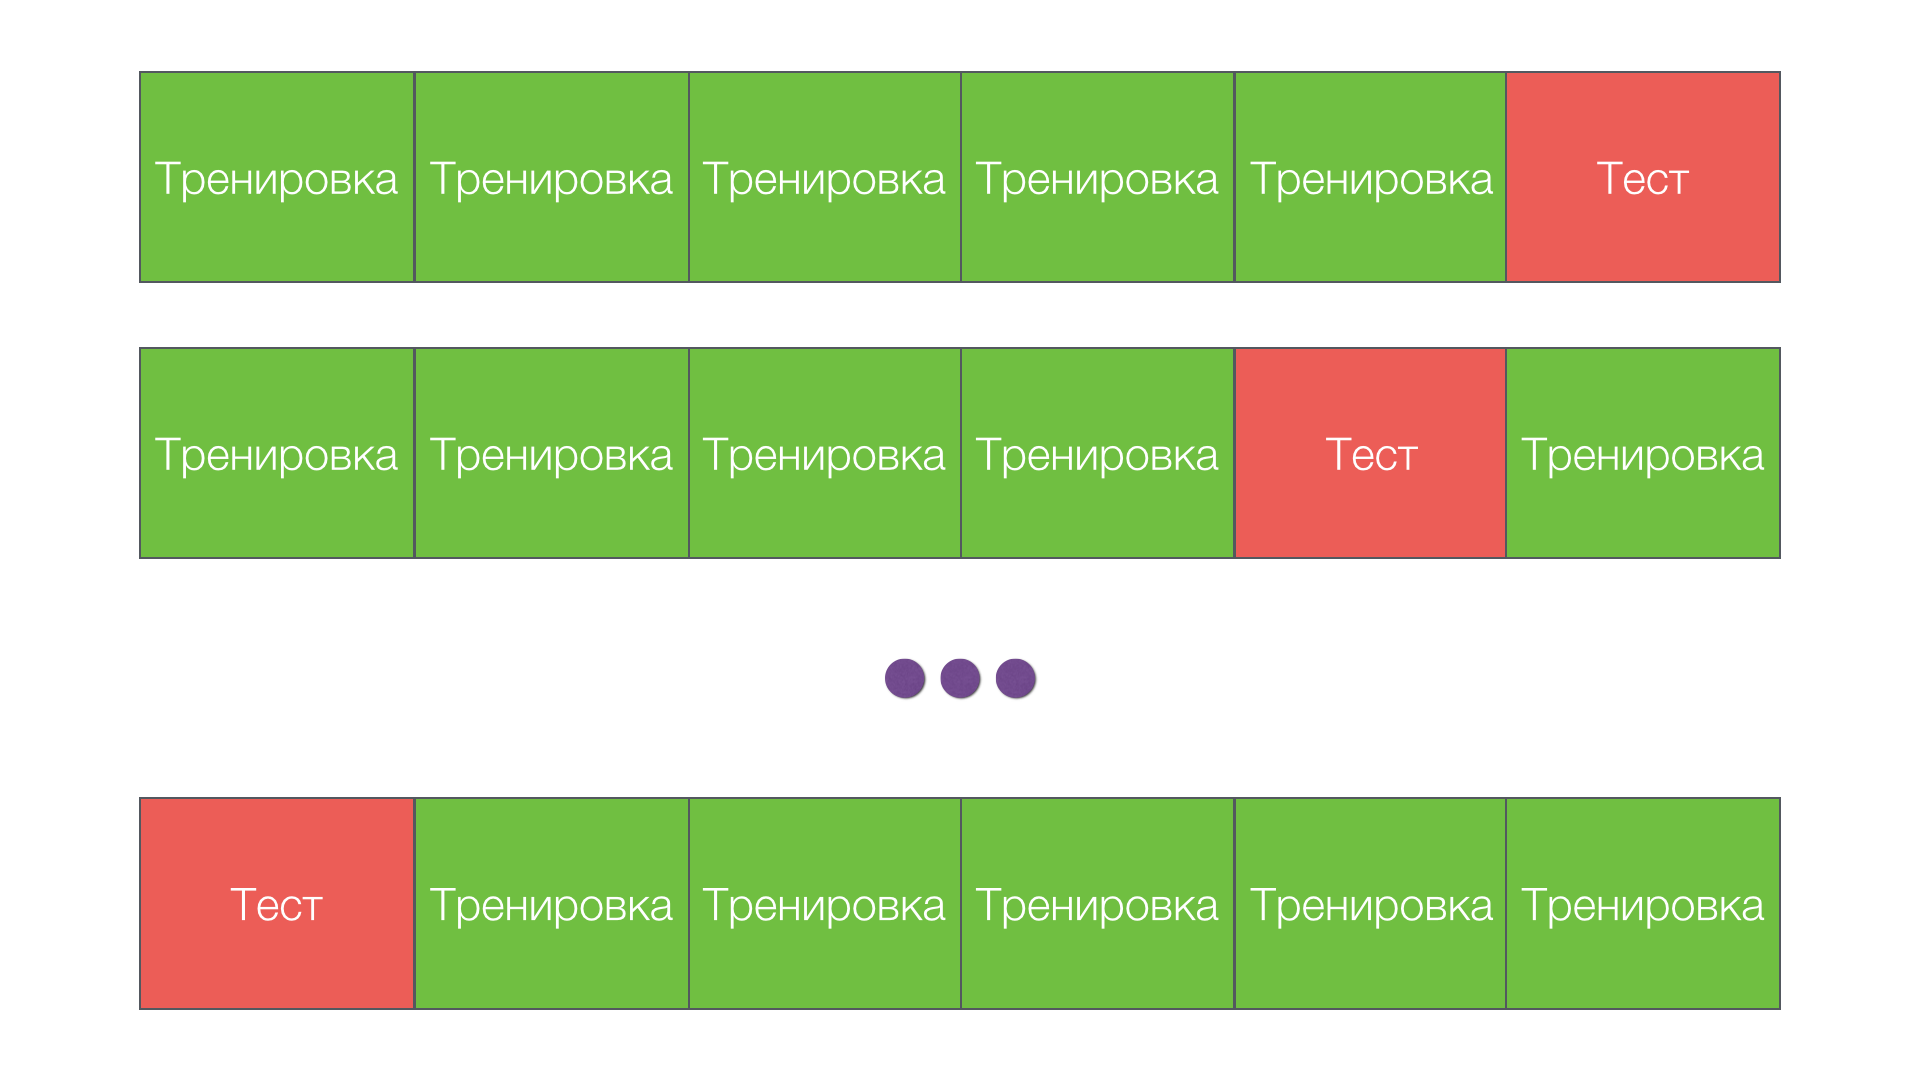
\includegraphics[scale=0.15]{images/cv.png}
\end{center}

частный случай: leave-one-out
  
\end{frame}

\begin{frame}{Решение 3: bootstrap}

выбираем в тренировочную выбоку $n$ объектов с возвращением

\begin{center}
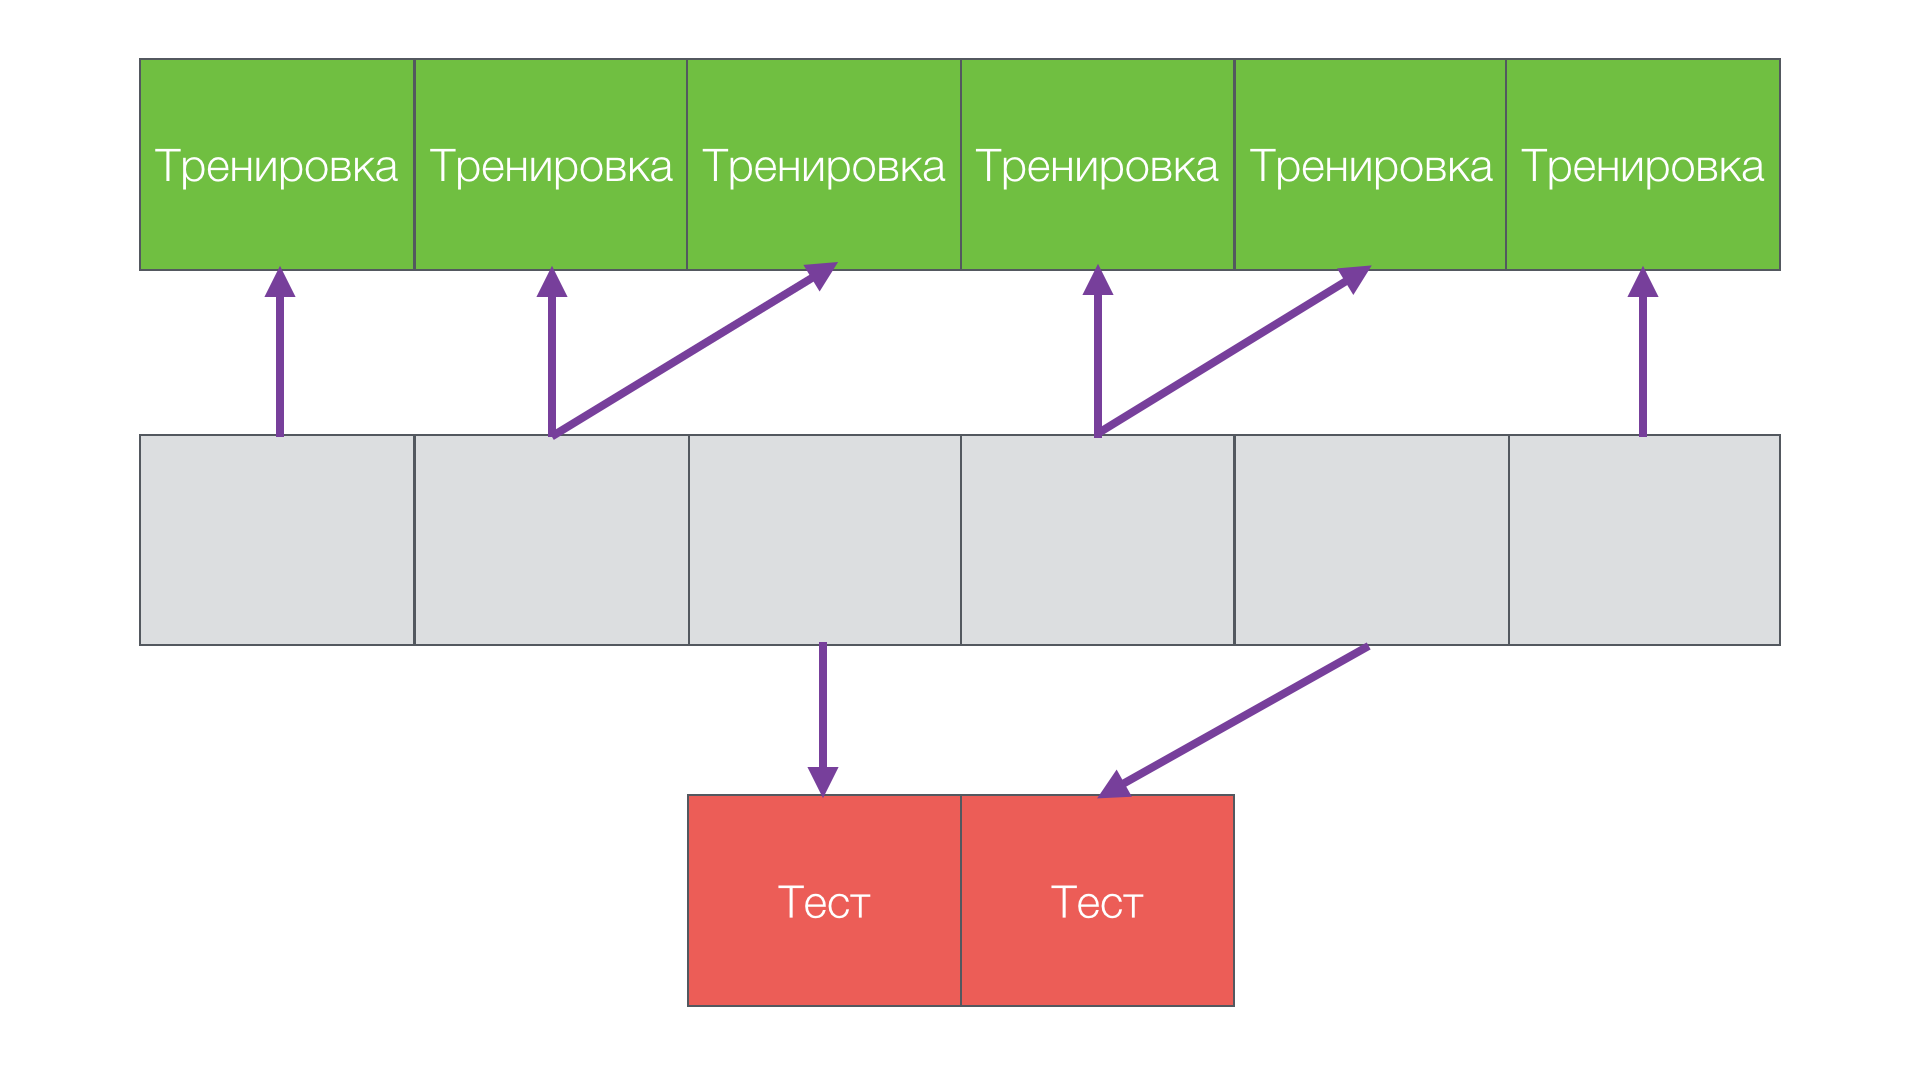
\includegraphics[scale=0.15]{images/boot.png}
\end{center}

упражнение: найти математическое ожидание размера тестовой выборки.
  
\end{frame}

\begin{frame}{Доверительный интервал для success rate}

При тестировании на $N=100$ объектах было получено $25$ ошибок. Таким образом измеренная вероятность успеха (success rate) составила $f=0.75$. Найти доверительный интервал для действительной вероятности успеха c уровнем доверия $\alpha=0.8$. 

\begin{exampleblock}{Решение}
Пусть $p$ -- действительная вероятность успеха в испытаниях бернулли, тогда
\[
f \sim \mathcal{N}\left( p, p(1-p)/N \right).
\]
Воспользовавшись табличным значением $P(-z \leq \mathcal{N}(0,1) \leq z) = \alpha$, имеем
\[
P\left(-z \leq \frac{f-p}{\sqrt{p(1-p)/N}} \leq z \right) = \alpha,
\]
откуда
\[
p \in \left(f + \frac{z^2}{2N} \pm z \sqrt{\frac f N - \frac{f^2}{N}+\frac{z^2}{4N^2}} \right)/\left(1 + \frac {z^2}{N} \right) = [0.69, 0.80]
\]
\end{exampleblock}
  
\end{frame}

\begin{frame}{Метрики качества. Вероятностные модели.}

Пусть $y_i$ - действительный класс для объекта $\mathbf{x}_i$
\begin{itemize}
\item  Information loss 
\[
- \frac 1 N \sum_i \log_2 p(y_i | \mathbf{x}_i)
\]
\item Quadratic loss 
\[
\frac 1 N \sum_j (p(y_j | \mathbf{x}_i) - a_j(\mathbf{x}_i))^2,
\] 
где
\[
a_j(\mathbf{x}_i) = \begin{cases}
1, \;\text{если}\;C_j = y_i\\
0, \;\text{иначе}
\end{cases} 
\]
\end{itemize}

\end{frame}

\begin{frame}{Метрики качества. Функции решения.}

\begin{center}
\begin{tabular}{|c r | c c|}
\cline{3-4}
 \multicolumn{2}{c|}{} & \multicolumn{2}{c|}{Предсказанный} \\
 \cline{3-4}
 \multicolumn{2}{c|}{} & {\bf true} & {\bf false} \\
 \hline
 \multirow{2}{*}{Действительный} & \multicolumn{1}{|c|}{\bf true} & TP & FN \\
 & \multicolumn{1}{|c|}{\bf false}  & FP & TN \\
 \hline
\end{tabular}
\end{center}

\[
success\;rate = accuracy = \frac{TP + TN}{TP + FP + FN + TN}
\]
\[
recall = TPR = \frac{TP}{TP + FN};\;\;precision = \frac{TP}{TP + FP}
\]
\[
FPR = \frac{FP}{FP + TN}
\]
\[
affinity = lift = \frac{accuracy}{p}
\]

\end{frame}

\begin{frame}{Receiver Operating Characteristic}

\[
TPR = \frac{TP}{TP + FN};\;\;FPR = \frac{FP}{FP + TN}
\]

\begin{center}
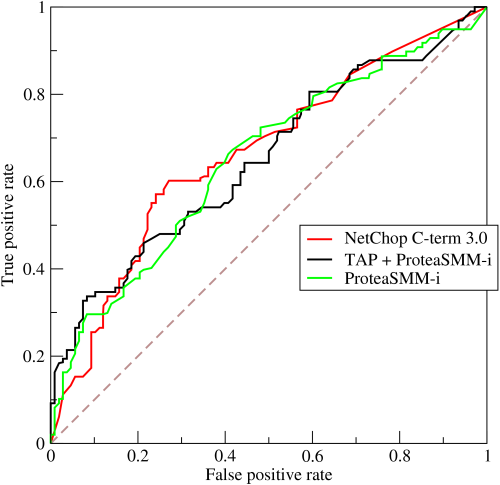
\includegraphics[scale=2.0]{images/roc.png}
\end{center}

\end{frame}

\begin{frame}{Упражнение}

\begin{exampleblock}{Простые классификаторы}
В генеральной совокупности существуют объекты 3 классов, вероятность появления которых $p_1 < p_2 < p_3$. Первый классификатор относит все объекты к классу с большей вероятностью (то есть к третьему). Второй классификатор случайно относит объект к одному из классов в соответствии с базовым распределением. Рассчитать precision и recall, которые эти классификаторы дают для каждого из 3 классов.
\end{exampleblock}

\end{frame}

\begin{frame}{Метрики качества. Регрессия}

\[
MSE = \frac 1 N \sum (h(\mathbf{x}_i) - y_i)^2, \;\; RMSE = \sqrt{MSE}
\]
\[
MAE =  \frac 1 N \sum |h(\mathbf{x}_i) - y_i|, \;\; RMAE = \sqrt{MAE}
\]
\[
RSE =  \frac{\sum (h(\mathbf{x}_i) - y_i)^2}{\sum (y_i - \bar{y})^2}
\]
\[
correlation = \frac{S_{hy}}{\sqrt{S_h S_y}};\;\; S_{yh} = \frac{\sum(h(i)-\overline{h(i)})(y_i - \bar y)}{N-1}
\]
\[
S_{h} = \frac{\sum(h(i)-\overline{h(i)})^2}{N-1};\;\;S_{y} = \frac{\sum(y_i - \bar y)^2}{N-1}
\]

\end{frame}

\begin{frame}{NFLT, MDL, AIC и все такое}

\begin{block}{No free lunch theorem}
Не существует единственной лучшей модели, решающей все задачи
\end{block}

\begin{block}{Minimum description length}
Лучшая гипотеза о данных -- та, которая ведет к самому краткому их описанию
\end{block}
\begin{block}{Akaike information criterion (AIC)}
\[
model = \arg\max	\ln p(\mathcal{D} | \theta_{ML}) - \|\theta\|
\]
\end{block}

\end{frame}

% ========================================
\section{Деревья решений}
% ========================================

\begin{frame}{}

\begin{center}
\Large Деревья решений
\end{center}

\end{frame}

\begin{frame}{Задача}

\begin{columns}[T]
    \begin{column}{.5\textwidth}
    {\bf Дано:}
    
		обучающая выборка из профилей нескольких десятков тысяч человек
		\begin{itemize}
		\item пол (binary)
		\item возраст (numeric)
		\item образование (nominal)
		\item и еще 137 признаков
		\item наличие интереса к косметике
		\end{itemize} 

	{\bf Задача:}

	Для рекламной кампании определить, характеристики людей, интересующихся косметикой
     
    \end{column}
    \begin{column}{.5\textwidth}
    
\includegraphics[scale=0.23]{images/nicole.jpg}    
    \end{column}
  \end{columns}
  
\end{frame}

\begin{frame}{Обама или Клинтон?}

\begin{center}
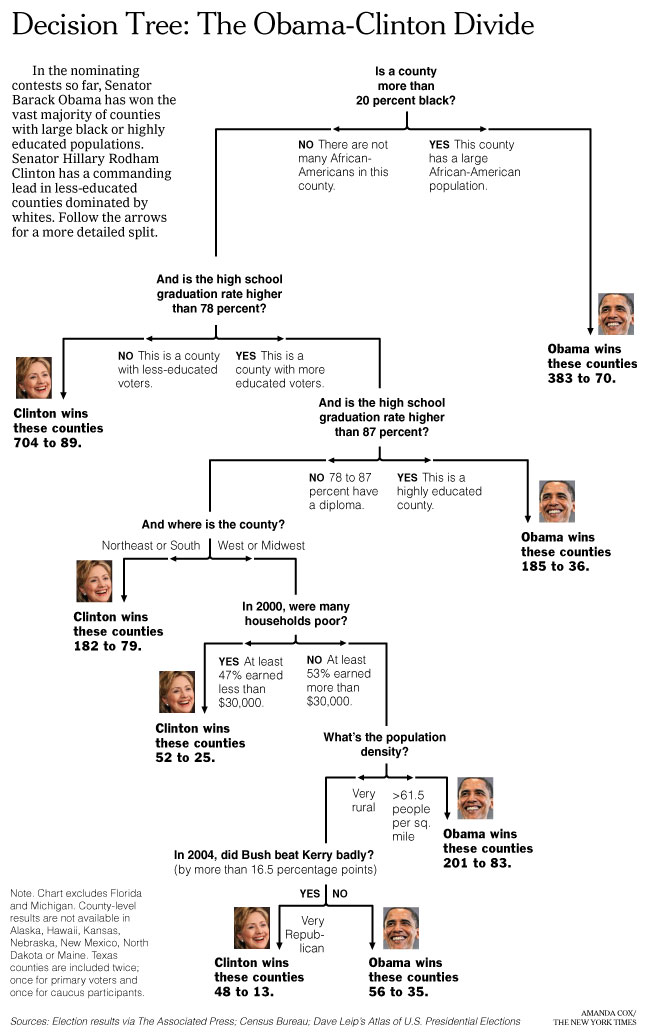
\includegraphics[scale=0.33]{images/obama.jpg}
\end{center}

\end{frame}

\begin{frame}{Хороший день для партии в гольф}

\begin{center}
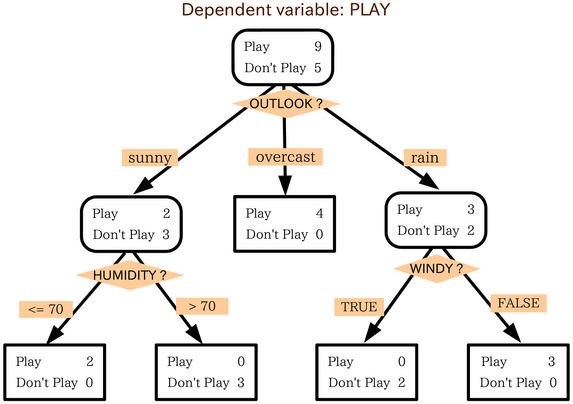
\includegraphics[scale=0.33]{images/golf.png}
\end{center}

\end{frame}

\begin{frame}{Регионы принятия решений}

\begin{center}
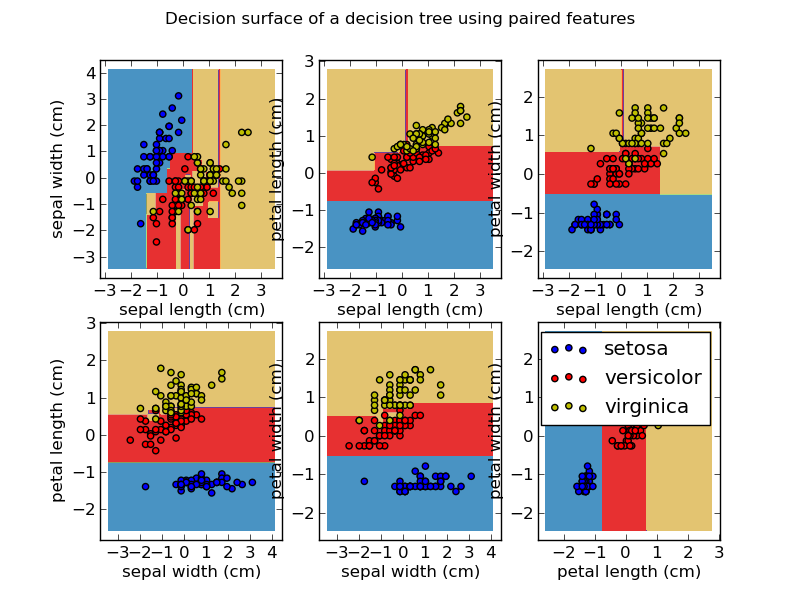
\includegraphics[scale=0.45]{images/regions.png}
\end{center}

\end{frame}

\defverbatim[colored]\dt{%
\begin{lstlisting}[tabsize=4,basicstyle=\ttfamily]
function decision_tree(X_N):
	if X_N satisfies leaf criterion:
		L = create_leaf(X_N)
		assign_class(L)
	else:
		L = create_node(X_N)
		X_1,..,X_S = split(L)
		for i in 1..S:
			C = decision_tree(X_i)
			add_child(L, C)
	return L
\end{lstlisting}
}

\begin{frame}{Рекурсивный алгоритм}

\dt

\end{frame}

\begin{frame}{CART}

Classification And Regression Trees

\begin{enumerate}
\item Как происходит разделение?
\item На сколько детей разделять каждый узел?
\item Какой критерий листа выбрать?
\item Как укоротить слишком большое дерево?
\item Как выбрать класс каждого листа?
\item Что делать, если часть значений отсутствует?
\end{enumerate}

\end{frame}

\begin{frame}{Чистота узла}

\begin{block}{Задача}
Выбрать метод, позволяющий разделить узел на два или несколько детей наилучшим образом
\end{block}

\vspace{1em}
Ключевое понятие -- {\it impurity} узла.
\begin{enumerate}
\item Misclassification
\[
i(N) = 1 - \max_k p(x \in C_k)
\]
\item Gini
\[
i(N) = 1 - \sum_k p^2(x \in C_k) = \sum_{i \neq j} p(x \in C_i) p(x \in C_j)
\]
\item Информационная энтропия
\[
i(N) =  -\sum_k p(x \in C_k) \log_2 p(x \in C_k)
\]
\end{enumerate}

\end{frame}

\begin{frame}{Теория информации}

Количество информации $\thicksim$ ``степень удивления''
\[
h(x) = -\log_2 p(x)
\]
Информационная энтропия $H[x] = E[h(x)]$
\[
H[x] = -\sum p(x) \log_2 p(x) \;\;\text{или}\;\; H[x] = - \int p(x) \log_2 p(x) dx
\]
\begin{exampleblock}{Упражнение}
Дана случайная величина $x$, принимающая 4 значения с равными вероятностями $\frac 1 4$, и случайная величина $y$, принимающая 4 значения с вероятностями $\{\frac 1 2, \; \frac 1 4, \; \frac 1 8, \; \frac 1 8\}$. Вычислить $H[x]$ и $H[y]$.
\end{exampleblock}

\end{frame}

\begin{frame}{Выбор наилучшего разделения}

\begin{block}{Критерий}
Выбрать признак и точку отсечения такими, чтобы было максимально уменьшение $impurity$
\[
\Delta i(N, N_L, N_R) = i(N) - \frac {N_L}{N} i(N_L) - \frac {N_R}{N} i(N_R)
\]
\end{block}

\vspace{1em}
Замечания
\begin{itemize}
\item Выбор границы при числовых признаках: середина?
\item Решения принимаются локально: нет гарантии глобально оптимального решения
\item На практике выбор impurity не сильно влияет на результат
\end{itemize}

\end{frame}

\begin{frame}{Если разделение не бинарное}

Естественный выбор при разделении на $B$ детей
\[
\Delta i(N, N_1, \ldots, N_B) = i(N) - \sum_{k=1}^B \frac{N_k}{N} i(N_k) \rightarrow \max
\]
Предпочтение отдается большим $B$. Модификация:
\[
\Delta i_B(N, N_1, \ldots, N_B) = \frac{\Delta i(N, N_1, \ldots, N_B)}{-\sum_{k=1}^B \frac{N_k}{N} \log_2 \frac{N_k}{N}} \rightarrow \max
\]
(gain ratio impurity)

\end{frame}

\begin{frame}{Использование нескольких признаков}

\begin{center}
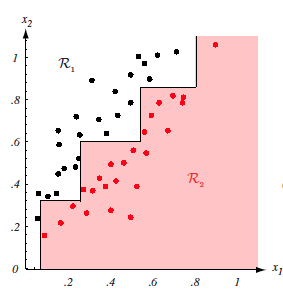
\includegraphics[scale=0.45]{images/multi1.png}\;
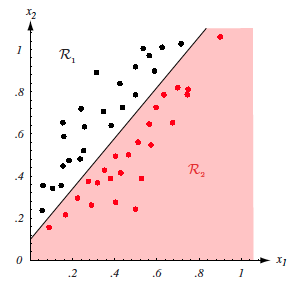
\includegraphics[scale=0.45]{images/multi2.png}
\end{center}

\end{frame}

\begin{frame}{Практика}

\begin{exampleblock}{Задача}
Вычислить наилучшее бинарное разделение корневого узла по одному признаку, пользуясь gini impurity.

\begin{center}
\begin{tabular}{| l | c | c | c | c |}
\hline
\textnumero & {\bf Пол} & {\bf Образование} & {\bf Работа} & {\bf Косметика} \\
\hline
1 & М & Высшее & Да & Нет \\
2 & М & Среднее & Нет & Нет \\
3 & М & Нет & Да & Нет \\
4 & М & Высшее & Нет & Да \\
1 & Ж & Нет & Нет & Да \\
2 & Ж & Высшее & Да & Да \\
3 & Ж & Среднее & Да & Нет \\
4 & Ж & Среднее & Нет & Да \\
\hline
\end{tabular}
\end{center}
\end{exampleblock}

\end{frame}

\begin{frame}{Когда остановить разделение}

Split stopping criteria
\begin{itemize}
\item никогда
\item использовать валидационную выборку
\item установить минимальный размер узла
\item установить порог $\Delta i(N) > \beta$
\item статистический подход
\[
\chi^2 = \sum_{k=1}^2 \frac{(n_{kL} - \frac{N_L}{N} n_{k})^2}{\frac{N_L}{N} n_{k}}
\]
\end{itemize}

\end{frame}

\begin{frame}{Укорачиваем дерево}

Pruning (a.k.a. отрезание ветвей)
\begin{enumerate}
\item Растим ``полное'' дерево $T_0$
\item На каждом шаге заменяем самый ``слабый'' внутренний узел на лист
\[
R_{\alpha}(T_k) = err(T_k) + \alpha size(T_k)
\]
\item Для заданного $\alpha $ из получившейся последовательности 
\[
T_0 \succ T_1 \succ \ldots \succ T_r
\]
выбираем дерево $T_k$, минимизирующее $R_{\alpha}(T_k)$
\end{enumerate}
Значение $\alpha$  выбирается на основании тестовой выборки или CV

\end{frame}

\begin{frame}{Какой класс присвоить листьям}

\begin{enumerate}
\item Простейший случай: \\ класс с максимальным количеством объектов
\item Дискриминативный случай: \\ вероятность $p(C_k | x)$
\end{enumerate}

\end{frame}

\begin{frame}{Вычислительная сложность}

Выборка состоит из $n$ объектов, описанных $m$ признаками

\vspace{1em}
Предположения
\begin{enumerate}
\item Узлы делятся примерно поровну
\item Дерево имеет $\log n$ уровней
\item Признаки бинарные
\end{enumerate}

\vspace{1em}
{\bf Обучение. } Для узла с $k$ обучающими объектами:

\vspace{1em}
\hspace{1em}Вычисление impurity по одному признаку $O(k)$

\hspace{1em}Выбор разделяющего признака $O(mk)$ 

\hspace{1em}Итог: $O(mn) + 2 O(m \frac{n}{2}) + 4 O(m \frac{n}{4}) + \ldots = O(m n \log n)$

\vspace{1em}
{\bf Применение. } $O(\log n)$

\end{frame}

\begin{frame}{Отсутствующие значения}

\begin{itemize}
\item Удалить объекты из выборки
\item Использовать отстутсвие как отдельную категорию
\item Вычислять impurity, пропуская отсутствующие значения
\item Surrogate splits: разделяем вторым признаком так, чтобы было максимально похоже на первичное разделение
\end{itemize}

\end{frame}

\begin{frame}{Surrogate split}
\vspace{-1em}
\[
c_1: \quad 
x_1=\begin{pmatrix}0 \\ 7 \\ 8\end{pmatrix},\;
x_2=\begin{pmatrix}1 \\ 8 \\ 9\end{pmatrix},\;
x_3=\begin{pmatrix}2 \\ 9 \\ 0\end{pmatrix},\;
x_4=\begin{pmatrix}4 \\ 1 \\ 1\end{pmatrix},\;
x_5=\begin{pmatrix}5 \\ 2 \\ 2\end{pmatrix}
\]
\[
c_2: \quad 
y_1=\begin{pmatrix}3 \\ 3 \\ 3\end{pmatrix},\;
y_2=\begin{pmatrix}6 \\ 0 \\ 4\end{pmatrix},\;
y_3=\begin{pmatrix}7 \\ 4 \\ 5\end{pmatrix},\;
y_4=\begin{pmatrix}8 \\ 5 \\ 6\end{pmatrix},\;
y_5=\begin{pmatrix}9 \\ 6 \\ 7\end{pmatrix}
\]
\begin{center}
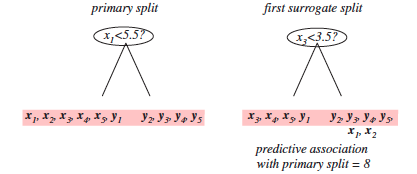
\includegraphics[scale=0.6]{images/surrogate2.png}
\end{center}

\begin{exampleblock}{Упражнение}
Вычислить второй surrogate split
\end{exampleblock}

\end{frame}

\begin{frame}{Задача о косметике}

\begin{center}
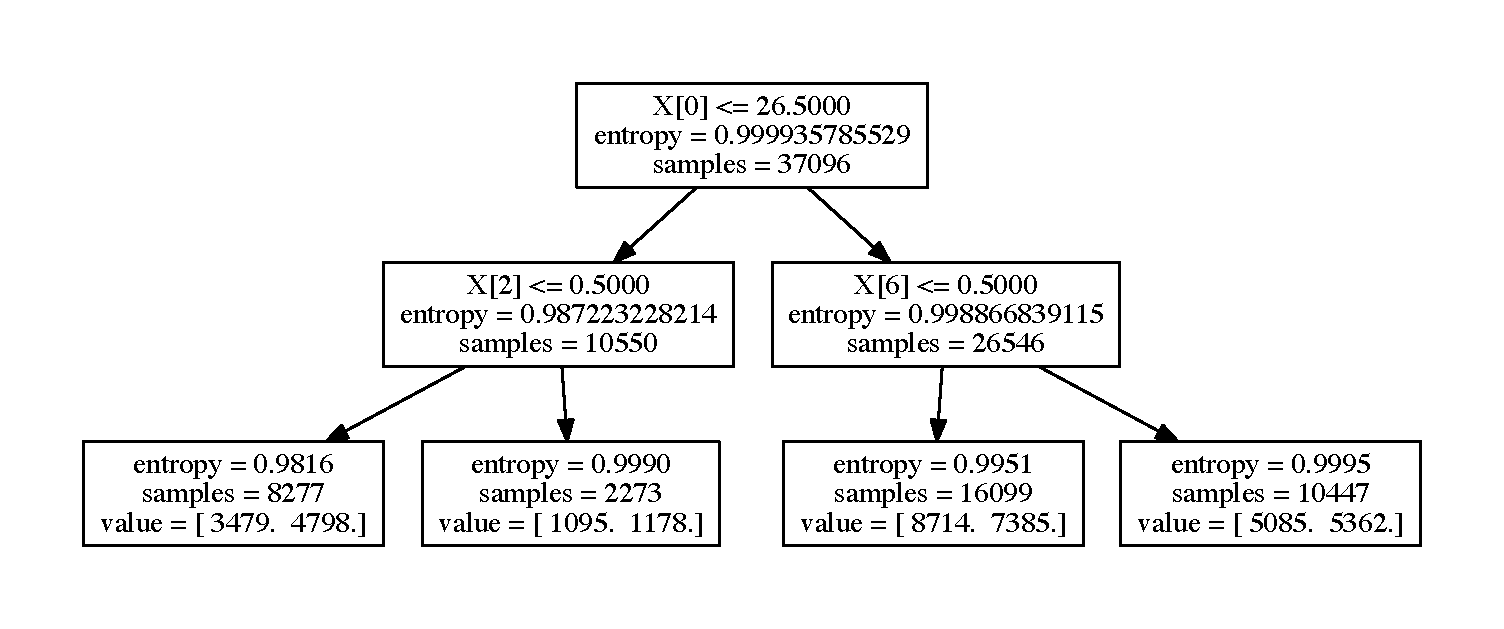
\includegraphics[scale=0.45]{images/model.pdf}
\end{center}

$X_0$ -- возраст, $X_4$ -- неоконченное высшее образование, $X_6$ - пол

\end{frame}

\begin{frame}{Задачи регрессии}

Impurity узла N
\[
i(N) = \sum_{y \in N} (y - \overline{y})^2
\]

Присвоение класса листьям
\begin{itemize}
\item Среднее значение
\item Линейная модель
\end{itemize}

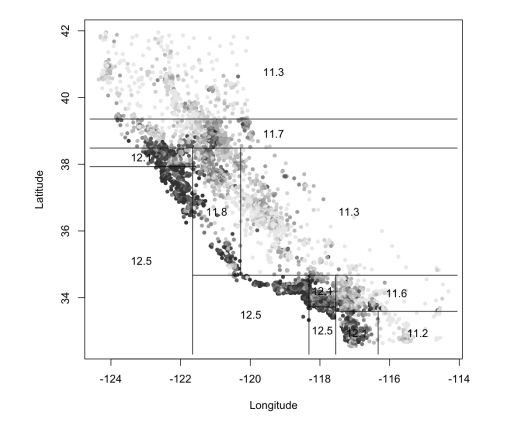
\includegraphics[scale=0.4]{images/housing.png}

\end{frame}

\begin{frame}{Кроме  CART}

\begin{itemize}

\item[ID3] Iterative Dichotomiser 3 
	\begin{itemize}
	\item Только номинальные признаки
	\item Количество детей в узле $=$ количество значений разделяющего признака
	\item Дерево растет до максимальной высоты
	\end{itemize}
	
\item[С4.5] Улучшение ID3
	\begin{itemize}
	\item Числовые признаки -- как в CART, номинальные -- как в ID3
	\item При отсутствии значения используются {\bf все} дети
	\item Укорачивает дерево, убирая ненужные предикаты в правилах
	\end{itemize}
	
\item[C5.0] Улучшение C4.5
	\begin{itemize}
	\item Проприетарный
	\end{itemize}
		
\end{itemize}

\end{frame}

\begin{frame}{Решающие деревья. Итог}

\begin{itemize}
\item[+] Легко интерпретируемы. Визуализация (ня!)
\item[+] Любые входные данные
\item[+] Мультикласс из коробки
\item[+] Предсказание за $O(\log n)$
\item[+] Поддаются статистическому анализу
\end{itemize}

\begin{itemize}
\item[--] Склонны к переобучению
\item[--] Жадные и  нестабильные
\item[--] Плохо работают при дисбалансе классов
\end{itemize}

\end{frame}

\begin{frame}{Ключевые фигуры}

\begin{columns}[T]
    \begin{column}{.5\textwidth}
    	\vspace{5em}
    	\begin{itemize}
			\item Claude Elwood Shannon \\ (Теория информации)
			\item Leo Breiman \\ (CART, RF)
			\item John Ross Quinlan  \\ (ID3, C4.5, C5.0)
		\end{itemize}        
    \end{column}
    \begin{column}{.5\textwidth}
    \begin{center}
    	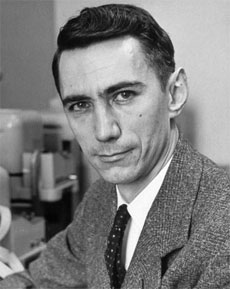
\includegraphics[scale=0.3]{images/shannon.jpg}\, 	   
	   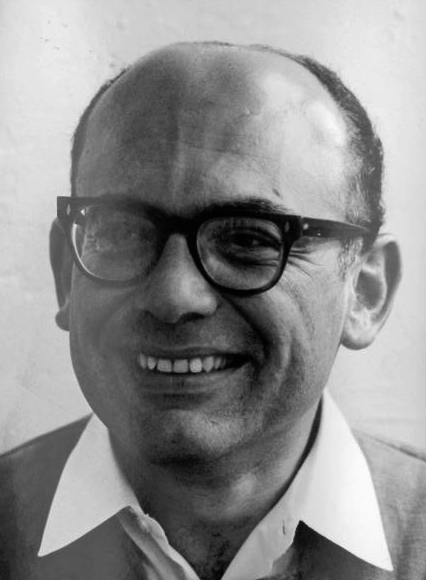
\includegraphics[scale=0.3115]{images/breiman.png}
	   	   
	   \vspace{0.3em}
	   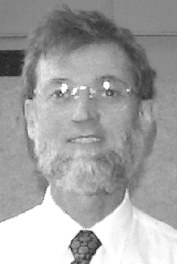
\includegraphics[scale=0.32]{images/quinlan.png} 
    \end{center}	   
    \end{column}
  \end{columns}

\end{frame}

\begin{frame}[plain]
\begin{center}
{\Large Вопросы}
\end{center}
\end{frame}

\end{document}